\documentclass[12pt,a4paper]{article}

\usepackage{datetime}
\usepackage{graphicx}
\usepackage{enumitem}
\usepackage{amsmath}
\usepackage{hyperref}
\usepackage{subcaption}

\title{Web Information System Project}
\newdate{date}{19}{06}{2020}
\date{\displaydate{date}}
\author{Nguyen Ngoc Lam - 20162316}

\begin{document}
\pagenumbering{gobble}
\begin{titlepage}
	\begin{center}
		\vspace*{0.5cm}
		\Huge
		\textbf{Web Information System Project}

		\vspace{0.5cm}
		\LARGE
		About How to Use VnPay to Transfer Money
            
		\vspace{1.5cm}

		\textbf{Nguyen Ngoc Lam - 20162316}

		\vfill
            
		A report presented what I have gained \\
		from doing this project
            
		\vspace{0.8cm}
     
		
\includegraphics[width=0.25\textwidth]{Logo_Hust.png}

		\Large
		School of Information and Communication\\
		Hanoi University of Science and Technology\\
		\displaydate{date}     
	\end{center}
\end{titlepage}
\newpage
\pagenumbering{arabic}
\tableofcontents
\newpage

\section{Overview about payment gateway}
\subsection{Payment gateway}
	\subsubsection{Definition}
	A payment gateway is a merchant service\footnote{refers to merchant processing services that enables a business to accept a transaction payment through a secure (encrypted) channel using the customer's credit card or debit card} provided by an e-commerce application service provider that authorizes credit card or direct payments processing for e-businesses, online retailers, bricks and clicks\footnote{a business model by which a company integrates both offline (bricks) and online (clicks) presences}, or traditional brick and mortar\footnote{refers to a physical presence of an organization or business in a building or other structure}. \\
	The payment gateway may be provided by a bank to its customers, but can be provided by a specialized financial service provider as a separate service, such as a payment service provider.\\
	A payment gateway facilitates a payment transaction by the transfer of information between a payment portal (such as a website, mobile phone or interactive voice response service) and the front end processor or acquiring bank\footnote{is a bank or financial institution that processes credit or debit card payments on behalf of a merchant like Visa or Master Card}
	Some payment gateways offer white label services, which allow payment service providers, e-commerce platforms, ISOs, resellers, or acquiring banks to fully brand the payment gateway’s technology as their own. This means PSPs\footnote{Payment Service Provider} or other third parties can own the end-to-end user experience without bringing payments operations,  and additional risk management and compliance responsibility, in house
	\subsubsection{Typical process}
	\begin{enumerate}
		\item Customer places an order on website.
		\item Encrypts the information to be sent between the user device and the merchant's web server.
		\item The merchant then forwards the transaction details to their payment gateway. This is another encrypted connection to the payment server hosted by the payment gateway. Some gateways allows users to bypass the merchant's web server and sent the information straight to them.
		\item The payment gateway converts the message from XML to  a message format\footnote{like ISO 8583} that understood by EFT Switches and then forwards the transaction information to the payment processor used by the merchant's acquiring bank.
		\item The payment processor forwards the transaction information to the card association\footnote{is a network of issuing banks and acquiring banks that process payment cards of a specific brand}
		\item The credit card issuing bank receives the authorization request, verifies the credit or debit available and then sends a response back to the processor (via the same process as the request for authorization) with a response code.
		\item The processor forwards the authorization response to the payment gateway.
		\item The payment gateway receives the response, and forwards it onto the interface that was used to process the payment, where it is interpreted as a relevant response, then relayed back to the merchant and cardholder. This is known as the Authorization or "Auth".
		\item The merchant then fulfills the order and the above process can be repeated but this time to "Clear" the authorization by consummating the transaction.
		\item The merchant submits all their approved authorizations, in a "batch" (end of the day), to their acquiring bank for settlement via its processor to reduced the number of "Clear".
		\item The acquiring bank makes the batch settlement request of the credit card issuer who makes a settlement payment to the acquiring bank (the next day in most cases).
		\item The acquiring bank subsequently deposits the total of the approved funds into the merchant's nominated account (the same day or next day).
	\end{enumerate}
	\subsubsection{Advantages over other payment methods}
	\begin{itemize}
		\item The merchant does not need to contact directly to bank thus can save time and human resource for them.
		\item Concentrating all the online transactions to a few gateway instead of each merchant have to create their own gateways.
		\item Safer than COD\footnote{Cash On Delivery} model for the merchants as they can ship the goods after the bank completed their verification.
		\item Less exchange of cash lead to faster and easier process for users since most of jobs was done behind a "closed door", where both customers and merchants cannot see.
		\item On a more recent note, reduced the human interactions thus preventing diseases from spreading.
	\end{itemize}
	\subsubsection{Disadvantages compared to other payment methods}
	\begin{itemize}
		\item Having an intermediate between you and the bank was never a good idea as they can see your information. If there was a security breach in the Payment gateway, your credit card information could be stolen.
		\item It is slower than a perfect COD scenario where the merchant can trust the customer to pay every time they order.
		\item Two encrypted connections from the firs few steps can be a target for hackers.
		\item The issue of credit card frauds is not addressed in the process. 
	\end{itemize}
\subsection{VnPay}
	\subsubsection{Overview}
	\begin{itemize}
		\item It is a payment gateway connecting merchants with banks.
		\item It allows customers to pay using credit/debit card, QR code and mobile banking applications on the phones.
	\end{itemize}
	\subsubsection{Benefits of using VnPay inside Vietnam}
	\begin{itemize}
		\item It is one of the most widely used payment medium in Vietnam.
		\item It has been incorporated into many mobile applications of popular banks like Vietcombank, BIDV and Vietinbank
		\item It has also been used in many e-wallets like viettelpay or VinID
		\item VnPayQR is supported by a lot of vendors in Vietnam
		\item It is easy to incorporated into your website by using code or by open-sourced plugins 
	\end{itemize}
	\subsubsection{How to incorporated}
	You can incorporated VnPay by 3 ways:
	\begin{enumerate}
		\item Through code: It delivered the most completed package but vendors need to have someone who can understand the demo code and how it works to deploy it.
		\item Through Third party open-sourced software: Vnpay has modules, libraries on third party open-sourced software like Magento, OpenCart and PrestaShop
		\item Through embedded code: Simple.
	\end{enumerate}
	\subsubsection{Deployment process}
	\begin{enumerate}
		\item Preparation
		\item Incorporated in test environment
		\item Testing
		\item Go live
	\end{enumerate}
	\subsubsection{Fee}
	Applied for all VnPayQR transactions
	\begin{itemize}
		\item For transaction using domestic card or bank account, e-wallet: 0.88\% of transaction value.
		\item For transaction using international credit/debit card: 2.2\% of transaction value.
	\end{itemize}
	Applied for all transactions using payment gateway:
	\begin{itemize}
		\item For transaction using domestic card or bank account, e-wallet: 1.1\% of transaction value with an additional fee of 1,650 Vietnam dong.
		\item For transaction using international credit/debit card: 2.2\% of transaction value with an additional fee of 2,500 Vietnam dong
	\end{itemize}
\section{Learning how to use VnPay through demo application}
\subsection{Language supported}
\begin{itemize}
	\item PHP
	\item C\#
	\item Python
	\item java
	\item NodeJS
	\item For this project, I will use python code.
\end{itemize}
\subsection{Configuration}
There are 2 configures to identify the website:
\begin{enumerate}
	\item vnp\_TmpCode: Website code on the VnPay server
	\item vnp\_HashSecret: Private code to authenticate (checksum) the server
\end{enumerate}
\subsection{Guide for incorporated}
\subsubsection{Create a payment URL}
Payment URL contains payment details like: what type of transactions it is, what bank does the customer use, what time do they send the request, How much is the transaction. 
\subsubsection{Code IPN URL}
IPN URl is used to get the result of processing the request on the server to the merchant using server-call-server call and the update/process the result will be done here.
\subsubsection{Code ReturnURL}
Vnpay sends data back to user by redirecting the browser to the website that the merchant provided. This site is used to show the result of the transaction to the end user
\subsection{Demo code}
\begin{figure}[h!]
	\centering
  	\begin{subfigure}[b]{\linewidth}
  		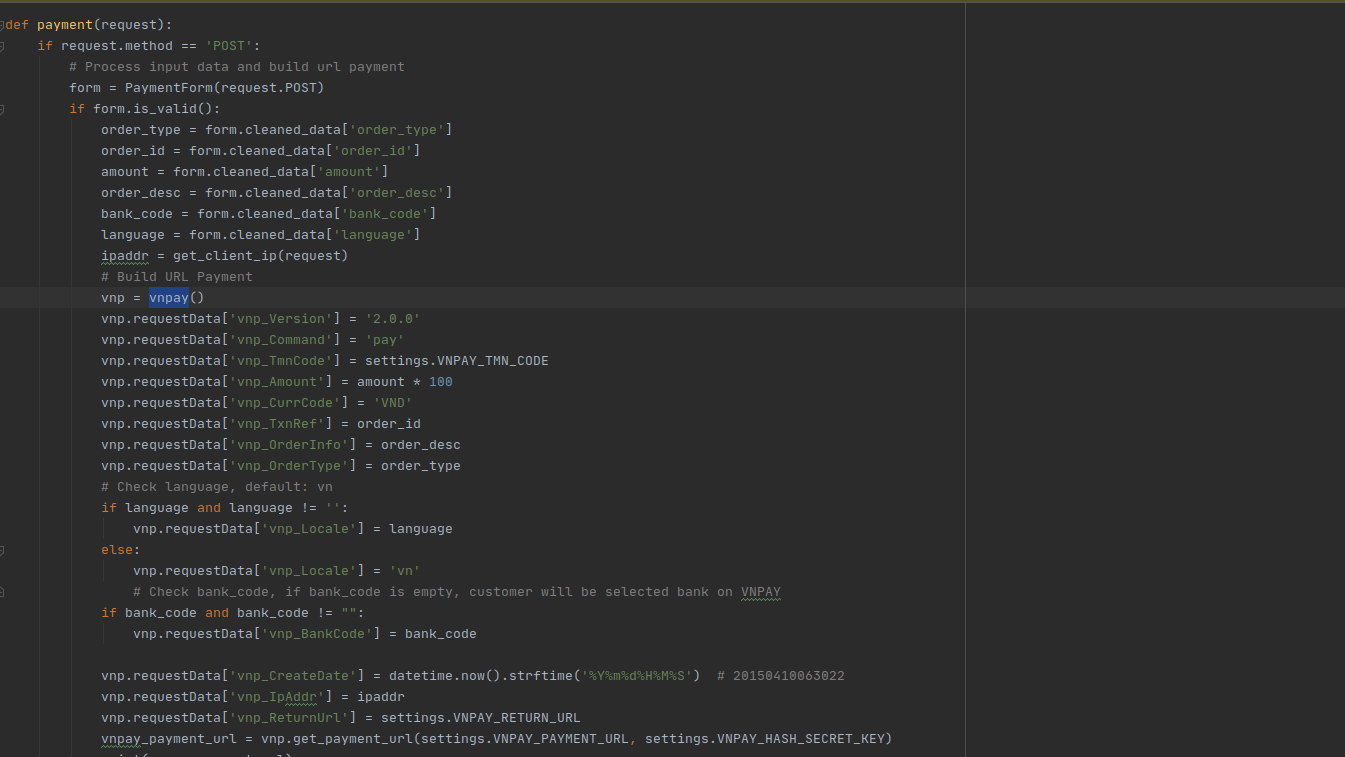
\includegraphics[width=\linewidth]{payment-1.png}
    	\caption{Render Payment URL parameter}
  	\end{subfigure}
  	\begin{subfigure}[b]{\linewidth}
    	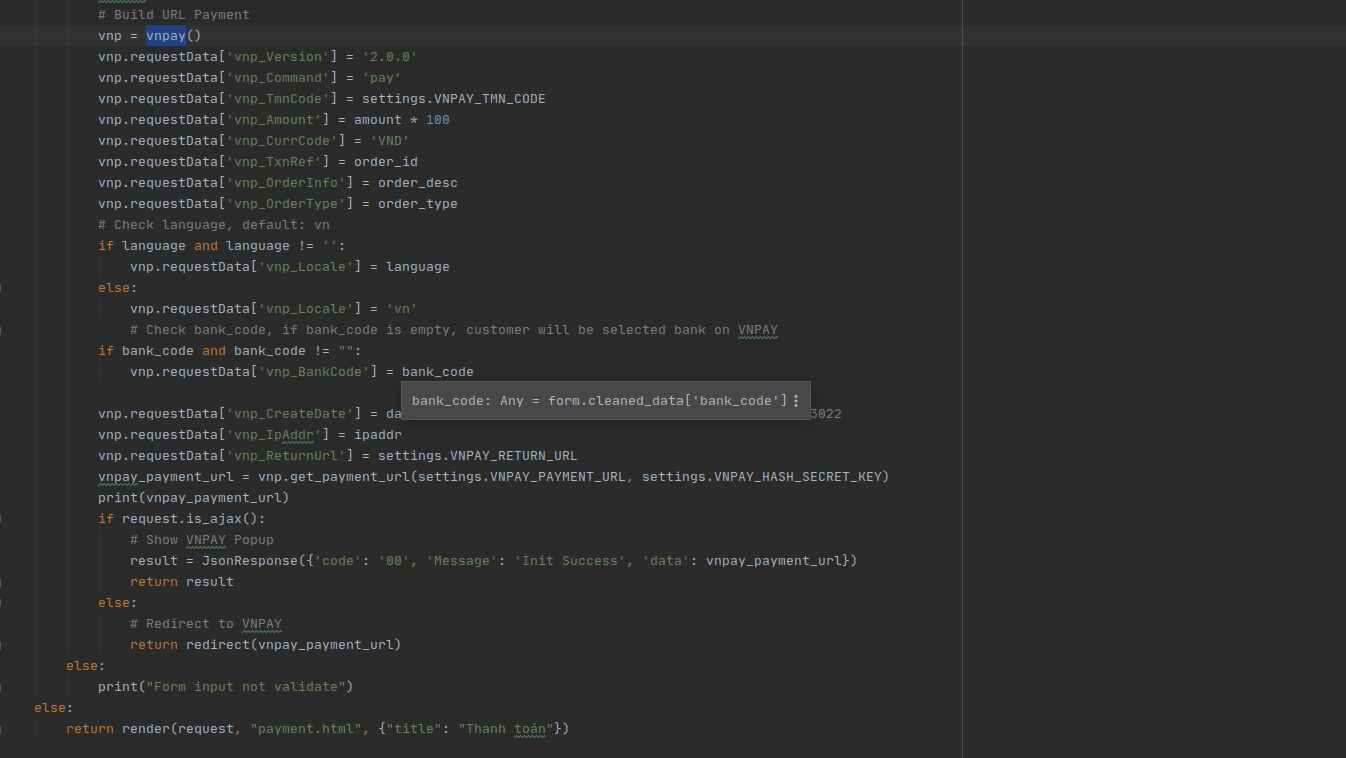
\includegraphics[width=\linewidth]{payment-2.png}
    	\caption{Return the full Payment URL}
  	\end{subfigure}
  	\caption{Create Payment URL}
  	\label{fig:purl}
\end{figure}

\begin{figure}[h!]
  	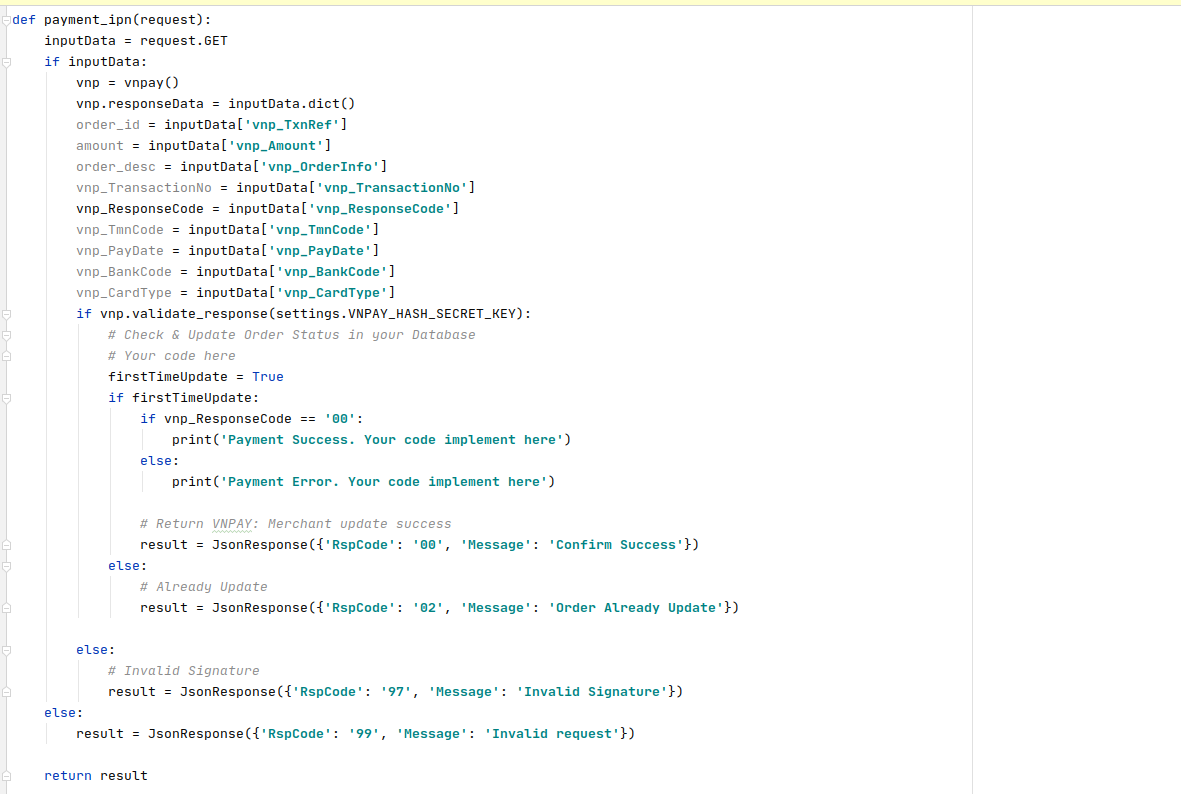
\includegraphics[width=\linewidth]{payment-ipn.png}
    \caption{Create IPN URL}
  	\label{fig:iurl}
\end{figure}

\begin{figure}[h!]
  	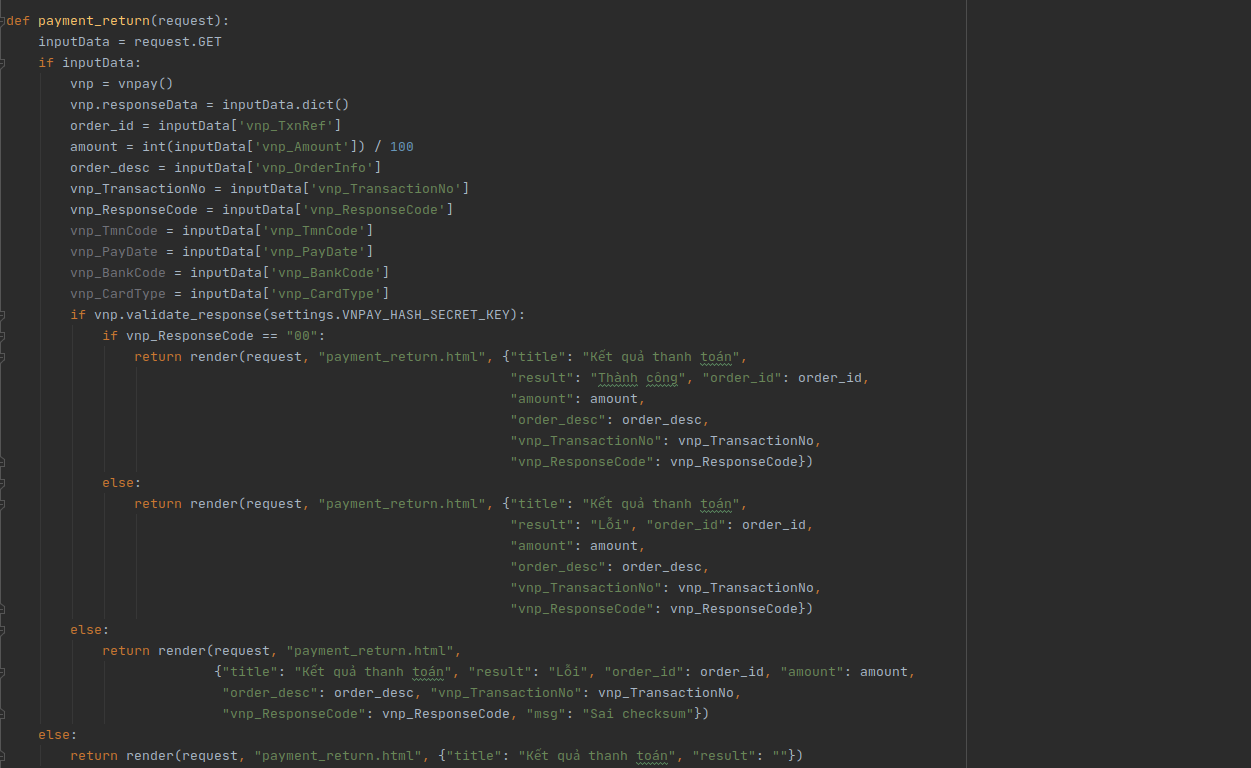
\includegraphics[width=\linewidth]{payment-re.png}
    \caption{Create ReturnURL}
  	\label{fig:rurl}
\end{figure}



\begin{thebibliography}{}
\bibitem{website}Payment gateway: \url{https://en.wikipedia.org/wiki/Payment_gateway}
\bibitem{website}Merchant services: \url{https://en.wikipedia.org/wiki/Merchant_services}
\bibitem{website}Bricks and clicks: \url{https://en.wikipedia.org/wiki/Bricks_and_clicks}
\bibitem{website}Brick and mortar: \url{https://en.wikipedia.org/wiki/Brick_and_mortar}
\bibitem{website}Acquiring bank: \url{https://en.wikipedia.org/wiki/Acquiring_bank}
\bibitem{website}Card association: \url{https://en.wikipedia.org/wiki/Card_association}
\bibitem{website}VnPay home page: \url{https://vnpay.vn/}
\bibitem{website}Payment gateway VnPay home page: \url{https://www.vnpayment.vn/}
\bibitem{website}VnPay features: \url{https://vnpayment.vnpay.vn/tinh-nang.htm}
\bibitem{website}VnPay fee: \url{https://vnpayment.vnpay.vn/phi.htm}
\bibitem{website}Documentation for API: \url{https://sandbox.vnpayment.vn/apis/docs/gioi-thieu/}
\end{thebibliography}

\end{document}